%
% requisitos.tex - padsoft 2014
% (c) 2014  M. Blanc, V. Macias
%

\documentclass[a4paper, 14pt]{article}

% español
\usepackage[utf8]{inputenc}
\usepackage[spanish]{babel}

% simbolos de euro
%\usepackage[official]{eurosym}
%\usepackage{newunicodechar}
%\newunicodechar{€}{\euro{}}

% diagramas y UML
%\usepackage{tikz}
%\usepackage{tikz-uml}
\usepackage[pdftex]{graphicx}
\DeclareGraphicsRule{.1}{mps}{*}{}
\DeclareGraphicsRule{.2}{mps}{*}{}

% estilos
\usepackage{enumitem}
\usepackage{titlesec}
\usepackage{graphicx}

% \parright
\SetLabelAlign{parright}{\parbox[t]{\labelwidth}{\raggedleft#1}}
%
\newenvironment{description-especial}
{\begin{description}[parsep=0pt, style=nextline]}
{\end{description}}

\newenvironment{description2}
{\begin{description}[style=multiline,topsep=10pt,leftmargin=4cm,font=\textbf, align=parright]}
{\end{description}}

\newcommand{\sectionbreak}{\clearpage}
%\titleformat{\section}{\huge\bfseries}{\thesection}{1em}{}
\usepackage[colorlinks=true,linkcolor=black,urlcolor=black]{hyperref}

% acronimos
%\newacronym{<label>}{<abbrv>}{<full>}

% titulo
\begin{titlepage}
	\title{Documento de análisis de requisitos}
	\author{M. Blanc \texttt{manuel.blanc@estudiante.uam.es}
		\and V. Macias \texttt{victor.macias@estudiante.uam.es}}
	\date{Viernes 7 de Febrero, 2014}
\end{titlepage}

\begin{document}

% tabla de contenidos
\clearpage\maketitle
\thispagestyle{empty}
\tableofcontents

\section{Introducción}
\subsection{Propósito del sistema}
El cliente ha encargado un paquete de software para administrar un videoclub.
En concreto, se busca automatizar el proceso de gestión de prestamos/devoluciones, proporcionando una interfaz gráfica.
El propósito de este documento es analizar el problema para ayudarnos a entender la situación, y llegar a un acuerdo con el cliente.

\subsection{Ámbito del sistema}
El software está dirigido principalmente a los empleados del videoclub.
El producto final debe permitir efectuar préstamos y devoluciones, y registrar a usuarios nuevos. Lo indispensable en general será:
\begin{itemize}
	\item Dar de alta socios. Para ello se le proporcionarán los datos requeridos, ya descritos, y el software devolverá un UID de socio.
	\item Efectuar préstamos de artículos, prestándolos durante un período de tiempo establecido por el gerente (en principio 3 días). Para ello:
	\begin{itemize}
		\item Se solicitará el UID de socio y se verificará tanto su existencia en la base de datos como que disponga de permisos para el préstamo. 
		\item Se buscará el artículo pedido. Para ello se ingresará el tipo de artículo y se buscará.
		\item Tras ello, se generará una transacción de compra en la que se seleccionará el tipo de pago, que podrá ser en efectivo o con tarjeta, y el socio deberá abonar el importe.
	\end{itemize}
	\item Vender contratos de tarifa plana de 30 días naturales. Un socio podrá comprar contratos de 1, 2 y 3 tipos de artículo distintos, que serán excluyentes para dicho socio. Además se podrá pagar un plus si el usuario quiere tener un día más de tarifa plana.
	\item Cambiar la disponibilidad de artículos deteriorados.
	\item Procesar devoluciones, verificando si el artículo a devolver tiene sanción. En caso de tener sanción, el software deberá generar una transacción con el importe a abonar. Hay dos niveles de sanción: sanción a corto plazo (antes de 10 días) y a largo plazo (a partir del día 10), con precios diferentes gestionados por el gestor.
\end{itemize}

Hemos considerado una serie de caracteristicas --no indispensables-- que pueden aportar valor adicional al producto final:
\begin{itemize}
	\item Contabilidad de la caja, quedando registro de todos los trámites en la aplicación. Esta mejora supone poder visualizar estos datos.
	\item Control de desperfectos. Es conveniente tener las sanciones unificadas en el sistema de devoluciones.
	\item Dar de baja socios. Los socios deberían poder solicitar que se borren sus datos de carácter personal de la base de datos.
\end{itemize}

Asimismo, tambien se ha acordado hacer ciertas omisiones en la funcionalidad del software para simplificarlo y reducir gastos.
\begin{itemize}
	\item Venta de películas viejas.
	\item Reservas. Es preferible que se gestionen por otra vía.
	\item Configuración del IVA. Los precios pueden ser ajustados manualmente y complica la interfaz.
\end{itemize}

%El fin del programa es que sea usado por los empleados del videoclub para asistirles con su trabajo.
%El sistema debe estar diseñado con esto en mente. Las labores propias de los empleados, en concreto efectuar préstamos y devoluciones. funcionamiento independiente.
%El sistema debe permitir controlar el stock y los prÉstamos. Además, debe permitir al gestor del videoclub obtener estadísticas sobre los clientes.
%El programa final debe ser independiente, y no deberá ser recopilado para añadir peliculas nuevas a la base de datos.

\subsection{Objetivos y criterios de éxito del proyecto}
El objetivo principal es facilitar la labor de los empleados.
Se considerara que el software ha alcanzado un nivel de funcionalidad básico cuando se puedan realizar las siguientes tareas dentro de un marco de tiempo razonable.
\begin{itemize}
	\item Registrar a un usuario nuevo en la base de datos.
	\item Efectuar un alquiler, denegando la operación si los datos necesarios no son válidos.
	\item Reiniciar la aplicación y comprobar que los datos son persistentes entre ejecuciones.
	\item Efectuar una devolución que lleve un retraso, y calcular correctamente la tasa de atraso.
\end{itemize}

\subsection{Definiciones, acrónimos y abreviaturas}
La aplicación debe representar una serie de objetos internamente.
A continuación estan definidas los campos que forman parte de cada una de las entidades lógicas.
Estos objetos los definimos como una tupla ordenada de los atributos que lo componen.

\subsubsection{Socios}
Se debe guardar toda la información necesaria para identificar a los socios, efectuar pagos y ponerse en contacto con ellos. Esta información es confidencial y debería estar guardada de manera segura.
\begin{description2}
	\item[UID]              Número de socio, aparecere en los carnéts emitidos (10 dígitos).
	\item[Nombre]           Nombre y apellidos del socio.
	\item[DNI/NIE]          Número de DNI completo, o alternativamente el NIE.
	\item[Dirección]        Dirección completa.
	\item[Teléfono]         Número de teléfono, móvil o fijo.
	\item[Email]            Dirección de correo electrónico. \textit{Opcional.}
\end{description2}

\subsubsection{Películas}
\begin{description2}
	\item[Título]           Título de la película.
	\item[Fecha]            Fecha de publicación.
	\item[Categorías]       Lista de categorías a las que pertenece.
	\item[Director]         Nombre del director.
	\item[Formato]          Formato de la película, puede ser DVD o Bluray.
	\item[Num. ejemplares]  Número de ejemplares \emph{total}.
\end{description2}

\subsubsection{Series}
\begin{description2}
	\item[Título]           Título completo de la serie.
	\item[Temporada]        Número de temporada.
	\item[Categorias]       Lista de categorias a las que pertenece.
	\item[Volumen]          Número de volumen. 
	\item[Formato]          Formato de la serie, puede ser DVD o Bluray.
	\item[Num. ejemplares]  Número de ejemplares \emph{total}.
\end{description2}

\subsubsection{Música}
\begin{description2}
	\item[Título]           Título completo del disco.
	\item[Géneros]          Géneros musicales a los que pertenece el disco.
	\item[Interprete]       Lista de interpretes, separada por comas.
	\item[Año]              Año de publicacion.
	\item[Formato]          Formato del disco, puede ser CD o vinilo.
	\item[Num. ejemplares]  Número de ejemplares \emph{total}.
\end{description2}


\section{Descripción del sistema}
\subsection{Requisitos funcionales}
Se debe hacer una distinción entre los empleados y el gerente del establecimiento.
Integracion con el SO.

\subsubsection{Tipo de usuario I: Empleado}
La interfaz de los empleados debe tener, obligatoriamente, al menos los siguientes elementos:
\begin{itemize}
	\item Un menú desde el que se pueda escoger el resto de opciones.
	\item Pantalla para dar de alta y baja socios.
	\item Pantalla de busqueda.
	\item Pantalla de pagos.
	\item Pantalla para hacer préstamos, debe tener búsqueda integrada.
	\item Pantalla de contratar tarifas VIP.
	\item Cambiar la disponibilidad de artículos deteriorados.
	\item Pantalla para devoluciones.
\end{itemize}

\subsubsection{Tipo de usuario II: Gerente}
El gerente de la tienda debe poder administrar la tienda desde la aplicación. Para acceder a esta funcionalidad, se debe proporcionar una contraseña. Su interfaz debe contener:
\begin{itemize}
	\item Pantalla para modificar los precios de alquiler de todas las categorías.
	\item Pantalla para crear y eliminar artículos nuevos en la base de datos.
	\item Visualización de la lista de morosos.
	\item Visualización de la lista de los articulos más solicidatos (top-ten).
\end{itemize}

\subsection{Requisitos no funcionales}
\subsubsection{Portabilidad}
El cliente puso especial énfasis es que la aplicación debe estar hecha en Java\texttrademark, y funcionar sobre Microsoft Windows\texttrademark.

\subsubsection{Accesibilidad}
Los empleados de la tienda no tienen por qué tener experiencia con ordenadores, y no deberían necesitar preparación para usar el software.

\subsubsection{Estabilidad}
El establecimiento maneja un volúmen considerable de alquileres mensualmente. El software debe poder almacenar un volúmen de datos considerable,aproximadamente 10.000 artículos entre las 3 categorias.

Además, el software debe garantizar la integridad de los datos en casos de uso normales.
En caso de error, el sistema debe manejarlo elegantemente.


\subsubsection{Seguridad}
Debe haber una jerarquía de permisos tal que los empleados no puedan acceder a acciones privilegiadas del gerente.

\section{Casos de uso}
Para ayudarnos a analizar el problema, hemos desarrollado casos concretos de uso de la aplicación.
Al tratarse de un sistema interactivo, es irreal pretender considerar todos los casos de uso.
En los siguientes ejemplos puede haber omisiones.

\subsection{Diagrama de casos de uso}
Este diagrama intenta resumir los posibles casos de uso de la aplicación:\\
{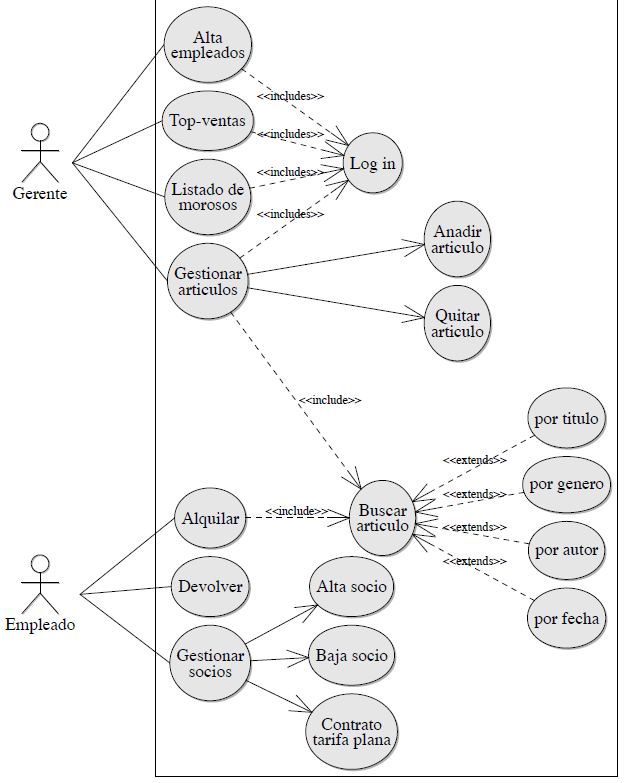
\includegraphics[width=14cm, height=14cm, keepaspectratio]{img/example.png}\\


\subsection{Descripción de casos de uso}
A continuación se detallan tres casos de uso que hemos estimado importantes: un alquiler, una devolución y una acción administrativa. El criterio que hemos seguido es la frecuencia de ocurrencia.
Para simplificar las descripciones y diagramas nos referiremos conjuntamente a películas, series y discos como artículos. Además, consideramos al empleado y socio como una misma entidad ya que los empleados solo actúan como nexo entre el socio y el software. 

\subsubsection{Préstamo}
\begin{description-especial}
	\item[Actor primario]         	\emph{Empleado}, atendiendo a \emph{socio}
	\item[Interesados y objetivos]	El socio desea alquilar un artículo, Smallville por ejemplo. El empleado debe procesar el trámite.
	\item[Precondiciones]         	El socio debe ser un socio registrado por el sistema.
	\item[Garantía de éxito (postcondiciones)] El socio alquila el artículo y el préstamo queda registrado en la aplicación.
	\item[Escenario principal de éxito] Interacciones del escenario, numeradas:
	\begin{enumerate}
		\item El empleado introduce el DNI/NIA del socio.
		\item El empleado busca el artículo solicitado, obteniendo el UID del artículo.
		\item Se verifica que los datos introducidos sean válidos, indicándoselo al empleado.
		\item El socio debe ahora abonar el importe del préstamo: efectivo o tarjeta.
		\item Se guarda un registro de la transacción y se genera la factura.
	\end{enumerate}
	\item[Extensiones (flujos alternativos)] Escenarios excepcionales:
	\begin{itemize}
		\item[3b.] El socio tiene cobros pendiente o artículos pendiente por devolver.
		\begin{enumerate}
			\item[i.]  El sistema no deja alquilar el artículo.
			\item[ii.] El empleado puede cancelar la operación.
		\end{enumerate}

		\item[3c.] El empleado no encuentra el artículo solicitado.
		\begin{enumerate}
			\item[i.] El empleado puede cancelar la operación.
		\end{enumerate}

		\item[4b.] El socio, por el motivo que alegue, desea cancelar la operación (no tiene dinero por ejemplo.)
		\begin{enumerate}
			\item[i.] El empleado puede cancelar la operación.
		\end{enumerate}
	\end{itemize}

	\item[Requisitos especiales] Tiempo de respuesta en la búsqueda de artículos moderadamente rápido.
	\item[Lista de variaciones de tecnología y datos] Ninguno
	\item[Frecuencia de ocurrencia] Entre 10 y 100 (depende del éxito del videoclub).
\end{description-especial}

\subsubsection{Devolución}
\begin{description-especial}
	\item[Actor primario]         	\emph{Empleado}, atendiendo a \emph{socio}
	\item[Interesados y objetivos]	Se desea devolver un artículo alquilado (volumen SmallVile)
	\item[Precondiciones]         	El socio debe ser un socio registrado por el sistema.
	\item[Garantía de éxito (postcondiciones)] El socio devuelve el artículo, Smallville, y el sistema detecta la devolución.
	\item[Escenario principal de éxito] Interacciones del escenario, numeradas:
	\begin{enumerate}
		\item El empleado introduce el DNI/NIA del socio y el UID del artículo.
		\item Se verifica que los datos introducidos sean válidos.
		\item El sistema se actualiza, marcando el artículo como disponible, e indicando que el socio ya no lo tiene.
	\end{enumerate}
	\item[Extensiones (flujos alternativos)] Escenarios excepcionales:
	\begin{itemize}
		\item[2b.] El socio ha devuelto el artículo fuera del período asignado.
		\begin{enumerate}
			\item[i.]  El sistema indica la cantidad a abonar. Si el socio no dispone del dinero solicitado, puede cancelar la operación pero seguirá teniendo la sanción y el artículo.
			\item[ii.] Si paga, el préstamo se devuelve y el sistema se actualiza.
		\end{enumerate}
	\end{itemize}

	\item[Requisitos especiales] Ninguno
	\item[Lista de variaciones de tecnología y datos] Ninguno
	\item[Frecuencia de ocurrencia] Entre 10 y 100 (depende del éxito del videoclub).
\end{description-especial}

\subsubsection{Registrar un socio nuevo}
\begin{description-especial}
	\item[Actor primario]                     	Empleado, Socio
	\item[Interesados y objetivos]            	Un individuo desea asociarse al videoclub
	\item[Precondiciones]                     	El cliente no debe estar registrado.
	\item[Garantía de éxito (postcondiciones)]	El cliente queda registrado como socio.
	\item[Escenario principal de éxito]       	Interacciones del escenario, numeradas:
	\begin{enumerate}
		\item El empleado introduce los datos del cliente.
		\item Se verifica que los datos introducidos sean validos.
		\item Los datos quedan guardados en la base de datos.
	\end{enumerate}
	\item[Extensiones (flujos alternativos)] Escenarios excepcionales:
	\begin{itemize}
		\item[2b.] El usuario ya está registrado.
		\begin{enumerate}
			\item[i.]  Se permite la posibilidad de cambiar los datos, o cancelar la operación.
		\end{enumerate}
	\end{itemize}

	Si el usuario ya esta registrado o los datos no son validos, el sistema notificara al empleado.
	\item[Requisitos especiales]                     	Ninguno.
	\item[Lista de variaciones de tecnología y datos]	Ninguno.
	\item[Frecuencia de ocurrencia] Entre 1 y 10 (depende del éxito del videoclub).
\end{description-especial}
\section{Maquetas}
A partir de toda la información reunida, hemos desarollado una maqueta de la interfaz de la aplicación. Se ha hecho a traves del IDE de NetBeans para que sea mas parecida al producto final. Solamente se mostrará de la parte del empleado, supóngase que la parte del gerente tendrá un aspecto muy parecido.\\

En primer lugar, el usuario sera bienvenido con la siguiente pantalla:\\
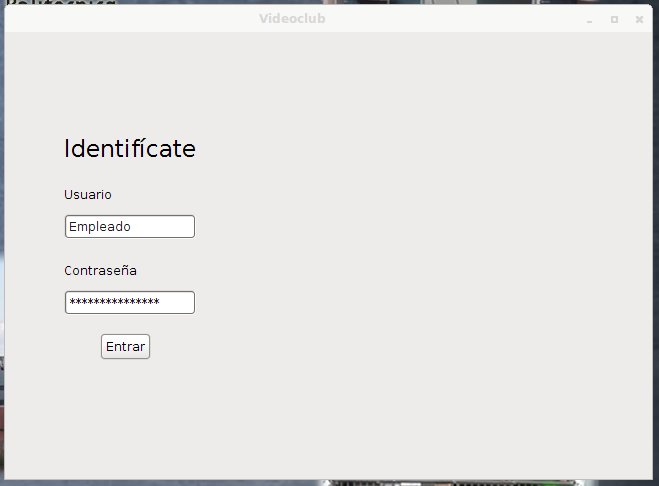
\includegraphics[width=10cm, height=10cm, keepaspectratio]{img/inicio.jpg}\\

Si el empleado quiere alquilar una película:\\
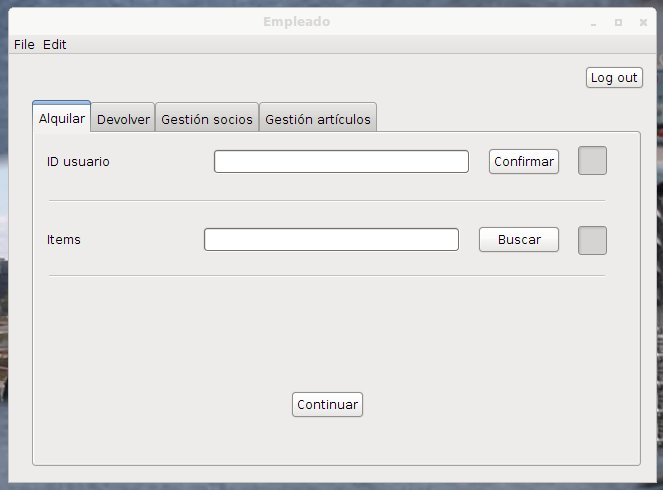
\includegraphics[width=10cm, height=10cm, keepaspectratio]{img/empleado-alquilar.jpg}\\
\clearpage

Primero ingresa la UID del socio. Luego, cuando el empleado busca el artículo, aparece la ventana de búsquedas:\\
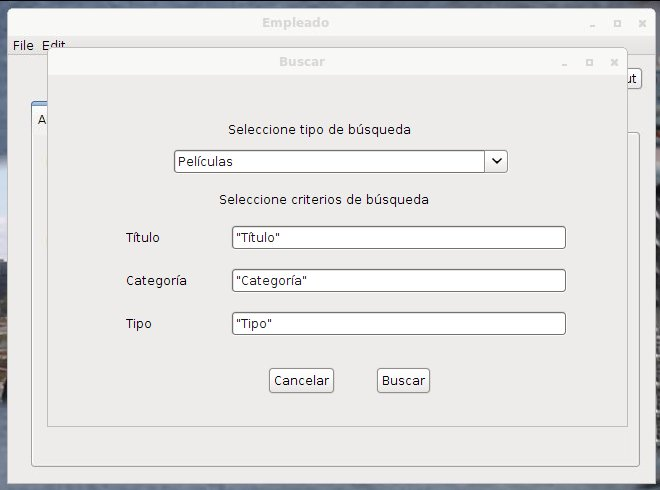
\includegraphics[width=10cm, height=10cm, keepaspectratio]{img/buscar-entrada.jpg}\\

Cuando el empleado tiene todos los datos de alquiler y le da a continuar, aparece la ventana de pago. En ella hay que seleccionar el método de pago:\\
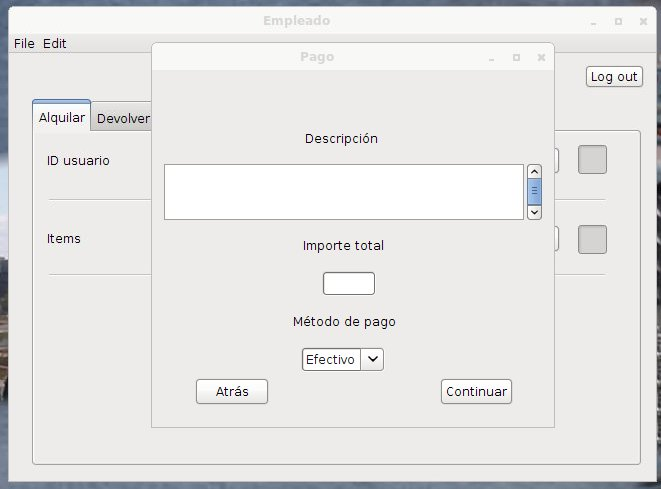
\includegraphics[width=10cm, height=10cm, keepaspectratio]{img/pagar.jpg}\\
\clearpage

Si el empleado quiere devolver una película, el menú será muy parecido al de alquiler:\\
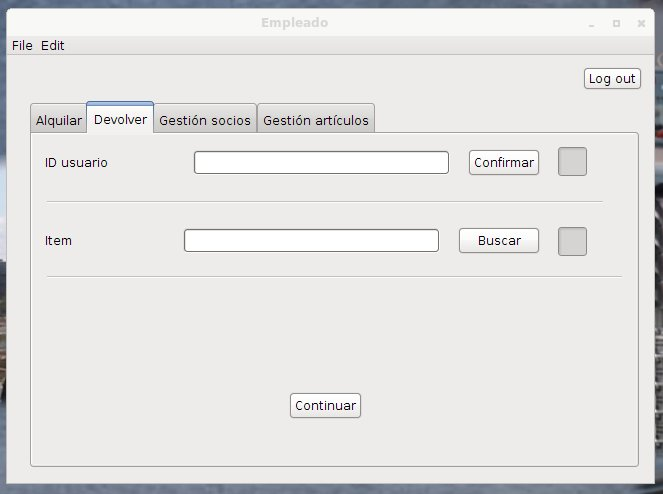
\includegraphics[width=10cm, height=10cm, keepaspectratio]{img/empleado-devolver.jpg}\\

Si el empleado accede a la gestión de socios, podrá dar de alta o de baja a socios, y contratar tarifas VIP:\\
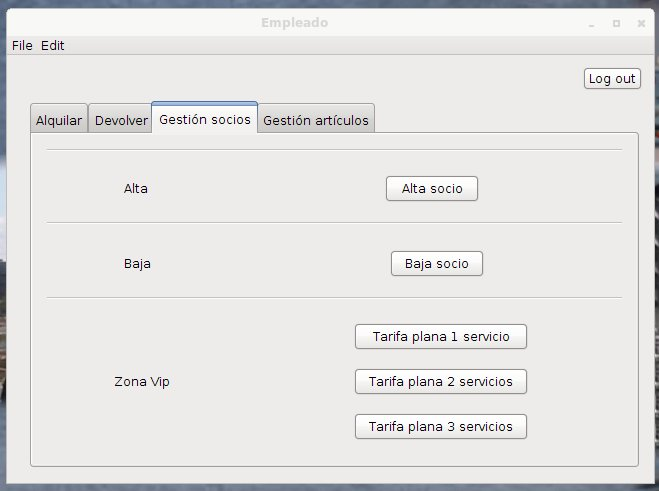
\includegraphics[width=10cm, height=10cm, keepaspectratio]{img/empleado-socios.jpg}\\
\clearpage

Si por ejemplo quiere dar de alta a un usuario, saldrá la siguiente ventana:\\
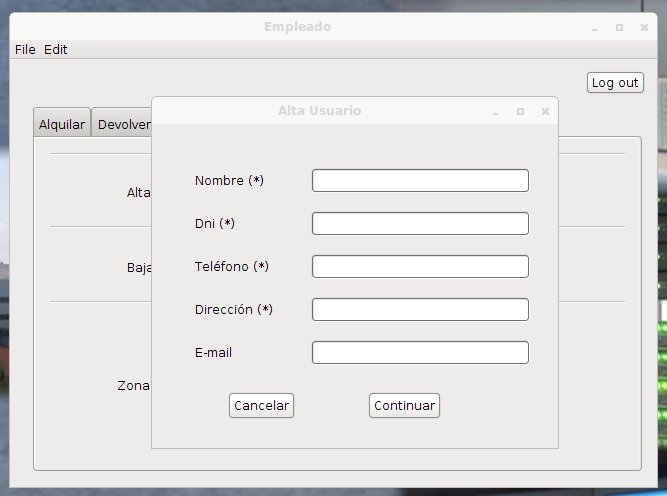
\includegraphics[width=10cm, height=10cm, keepaspectratio]{img/altasocio.jpg}\\

Si el empleado accede a la gestión de artículos, podrá añadir nuevos artículos y retirar alguno ya existente (aquí tambien podrá acceder el gerente):\\
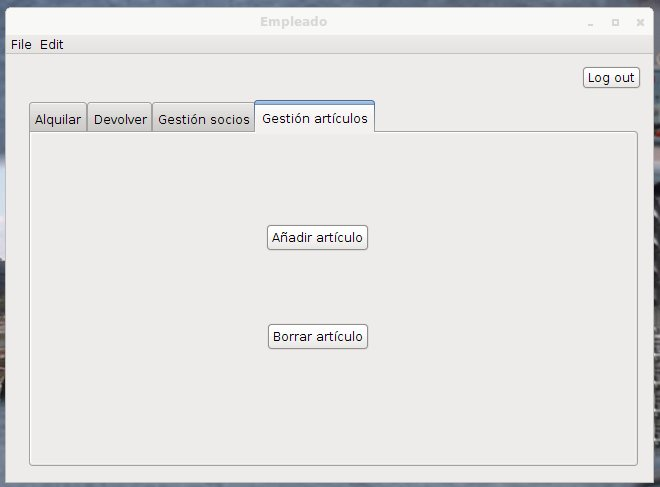
\includegraphics[width=10cm, height=10cm, keepaspectratio]{img/empleado-articulos.jpg}
\clearpage

Si el empleado quiere añadir un artículo al videoclub, saldrá la siguiente ventana:\\
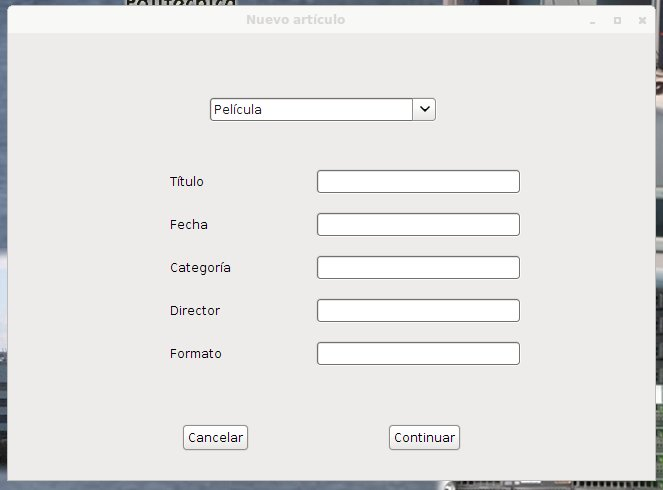
\includegraphics[width=10cm, height=10cm, keepaspectratio]{img/nuevoarticulo.jpg}\\
\clearpage

	

\section{Apéndice (OOC)}
Al elaborar este documento, nos hemos dado cuenta de que quedan aún muchos temas abiertos que habrá que concretar con el cliente.
Las entrevistas verbales son imprecisas, puede cambiar las especificaciones día a día.

Se nos olvidó preguntar al cliente el porqué quiere el sistema, y qué sistema estaba usando antes. Esto es muy importante para averiguar lo que el cliente verdaderamente necesita y no lo que quiere. 


\end{document}

